%%%%%%%%%%%%%%%%%%%%%%%%%%%%%%%%%%%%%%%%%%%%%%%%%%%%%%%%%%%%%%%%%%%%%%%
% Instructions: Comments in the file below indicate where the
% following steps have to be performed.
% Step 1: Enter abstract title.
% Step 2: Enter author information.
% Step 3: Enter key words.
% Step 4: Enter main text of abstract.
% Step 5: Enter references, e.g. using a simple list.
%%%%%%%%%%%%%%%%%%%%%%%%%%%%%%%%%%%%%%%%%%%%%%%%%%%%%%%%%%%%%%%%%%%%%%%
\documentclass[10pt,a4paper]{article}
%\usepackage{times}
%\usepackage{tgtermes}
%\usepackage[T1]{fontenc}
% sur un syst�me mac os utiliser la ligne suivante
%\usepackage[applemac]{inputenc}
% sur un syst�me windows utiliser la ligne suivante
%\usepackage[latin1]{inputenc}
% sur un syst�me linux en utf8 utiliser al ligne suivante
\usepackage[utf8]{inputenc}
\usepackage[english]{babel}
\usepackage{fancyhdr}
\usepackage{setspace}
\setstretch{1,15}
\usepackage{gensymb}
\usepackage{amsmath}
\usepackage{amsfonts}
\usepackage{amssymb}
\usepackage{graphicx}
\usepackage{xcolor}
\usepackage{wrapfig}

\usepackage{titlesec}
\titleformat{\section}
  {\normalfont\fontsize{16}{20}\bfseries}{\thesection}{1em}{}
\titleformat{\subsection}
  {\normalfont\fontsize{16}{20}\bfseries}{\thesubsection}{1em}{}
\titlespacing*{\section}
{0pt}{2.ex plus 1ex minus .2ex}{.0ex}
\titlespacing*{\subsection}
{0pt}{0.ex}{.0ex}

\setlength{\parindent}{20pt}
\setlength{\parskip}{5pt plus 2pt minus 1 pt}
\topmargin  -12mm
\evensidemargin 5mm
\oddsidemargin  0mm
\textwidth  158mm
\textheight 245mm
\headheight 14pt
\headsep 1.2cm

\pagestyle{fancy}
\rfoot{}
\chead{}
\cfoot{}
\lhead{
 \textit{Algorithmic modelling of multiphysic processes}}              
 \rhead{
  \textit{2020-2021}}


\begin{document}
%\pagestyle{empty}



\begin{center}
\begin{spacing}{2.05}
{\fontsize{20}{20}
\bf
% Step 1: Enter abstract title here.
Multiphysic study of Nb3Sn superconducting strand during heat treatment
}
\end{spacing}
\end{center}
\vspace{-1.95cm}
\begin{center}
{\fontsize{14}{20}
\bf
A. GORYNIN\textsuperscript{a}\\%, A. AUTEUR\textsuperscript{b}\\
\medskip
%\vspace{0.75cm}
}
{\fontsize{12}{20}
a. Endommagement, \quad arsenii.gorynin@ens-paris-saclay.fr\\
%b. Affiliation + email
}
\end{center}

\vspace{5pt}

{\fontsize{16}{20}
\bf
Abstract :
}
\bigskip

\textit{ Growth of intermetallics (IMCs) between Cu and Sn plays important role during the heat treatment of superconducting $Nb_3Sn$ wires. Here we present a simplified 1D model of diffusion controlled IMCs growth inside the sub-element of the wire. The external pressure effect on the rate of IMCs is considered by coupling with mechanical elasticity problem. }

\vspace{10pt}

{\fontsize{12}{20}
\bf
Keywords : Superconducting wires, heat treatment, diffusion controlled phase kinetics, finite differences, 1d model. 
}
%\bigskip

\section{Introduction}
\medskip

$Nb_3Sn$-based superconductors are widely used for production of powerful high-field electromagnets (greater than 10 T). Superconducting materials have no electrical resistance at cryogenic temperatures (a few K) and can therefore carry high currents to generate large magnetic inductions, while remaining compact and consuming little energy. 

The $Nb_3Sn$-based conductor is produced in rectangular Rutherford type cables, braided from strands. 
It is composed of a few dozen superconducting round wires twisted and flattened into a tape-like shape. These cables are then wound to form the coils of the electromagnet. After winding, the whole coil requires a heat treatment up to 650 $C^\circ$ in a controlled atmosphere. The reason for that is brittleness of Nb3Sn which means that to avoid the failure of the superconducting phase during the fabrication it is necessary to apply heat treatment after the winding. 

During heat treatment, various physico-chemical phenomena lead to the formation of the $Nb_3Sn$ superconducting phase in the sub-elements with the formation of the superconducting ring region inside the wire. The dynamics of the dimensional changes of the conductors is still poorly known, and if these dimensional changes are not taken into account by the tooling, mechanical stresses accumulate within the coils and degrade the superconducting performance of the conductor. A multiphysic study of the phenomena is thus interesting to understand the thermomechanical process of $Nb_3Sn$ conductors during heat treatment.  

There are several possible approaches for wire design and fabrication. Here we will condiser the Restacked Rod Process (RRP) design, which was developed by Oxford Superconducting Technology  in the early 2000s.
The geometry of the wire is arranged in such a way that inside the wire there is an ordered set of circular sub-elements embedded inside a copper matrix. 
Each sub-element has it's own diffusion barrier.  The main point of diffusion barriers is not to poison the main copper matrix.  In turn, each sub-element consists of a Sn core surrounded by a copper matrix. Nb filaments are located in a ring inside the copper matrix, with the  small distance between each filament.

The standard heat treatments scheme for RRP consists from 3 main steps. During the last step the final reaction of Nb and Sn takes place at the temperature around 650 $C^\circ$ with formation  of $Nb_3Sn$ ring.
At the first step of the heat treatment, diffusion between Cu and Sn occurs and nucleation and growth of IMCs takes place. The first step is also called mixing step.  After 48 hours at 215 $C^\circ$ temperature there is an unreacted Sn in the core, surrounded by a layer of $\eta$ ($Cu_6Sn_5$) phase and then a layer of $\varepsilon$ ($Cu_3Sn$) phase. 
In this study we will focus on IMCs kinetics between Cu an Sn during the first step of the heat treatment process (HTP).
\begin{figure}[h]
\begin{minipage}[h]{0.5\linewidth}
\center{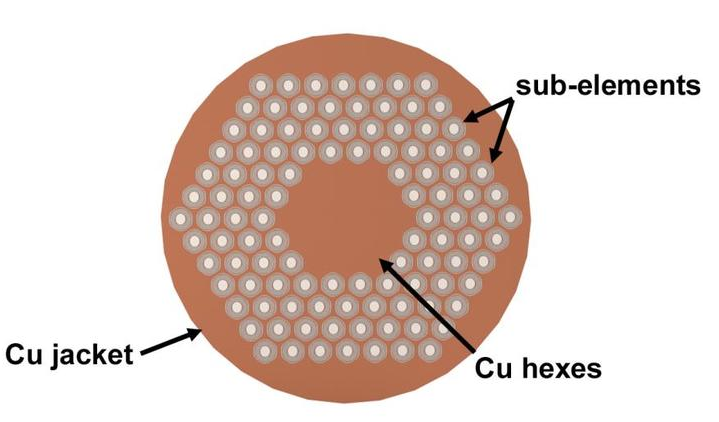
\includegraphics[width=1.1\linewidth]{images/RRP_1.png} }
\end{minipage}
\hfill
\begin{minipage}[h]{0.5\linewidth}
\center{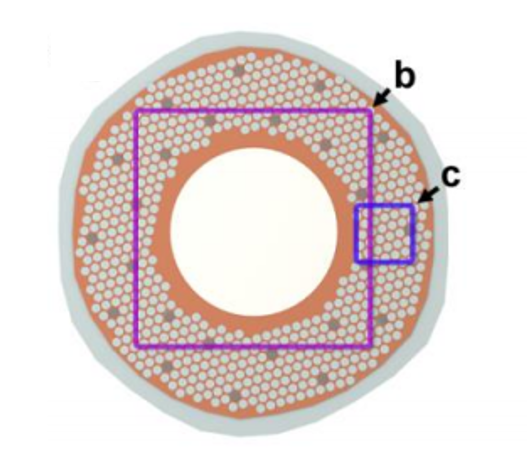
\includegraphics[width=0.8\linewidth]{images/RRP_2.png} }
\end{minipage}
\vspace{-2.5em}
\caption{Schematic representation of RRP wire cross-section (left). Sub-element cross-section (right).}
\end{figure}

\section{Model description}

\subsection{Geometry}

\begin{wrapfigure}{r}{0.35\textwidth}
\vspace{-3em}
  \begin{center}
    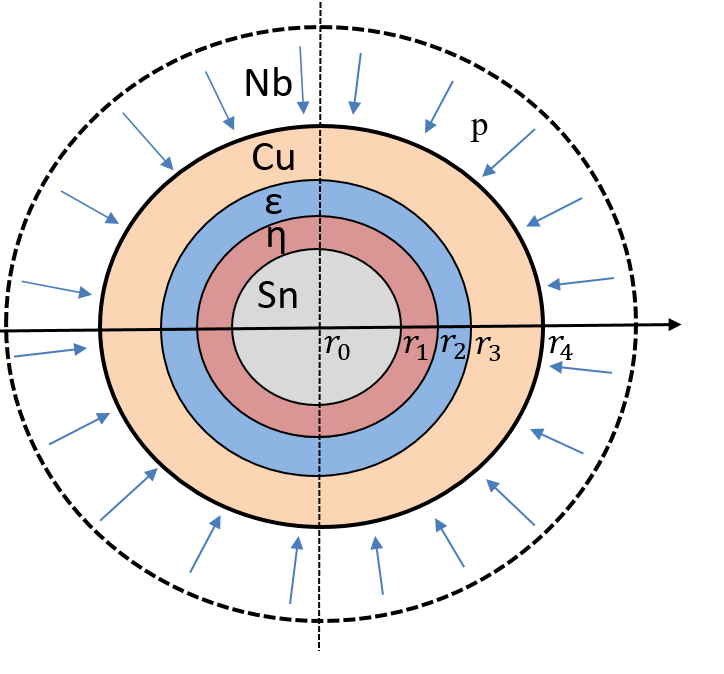
\includegraphics[width=0.4\textwidth]{images/prob_statement2.png}
\end{center}
\vspace{-2em}
\caption{\centering Simplified sub-element geometry.}
\end{wrapfigure}

The geometry of the representative sub-element is assumed to be axisymmetric as shown on Figure 2. 
At the first step, the diffusion between Cu and Sn takes place on the interface between Sn core and Cu matrix. Hence, we don't consider here the Nb filaments ring, as it's not participate in the process during the first step of HT. Plus we apply extenral pressure at the interface between Nb filaments and copper matrix. 
Our goal is to track IMCs evolution until it reach Nb ring.

We assume the presence of thin intermetallic layers from the beginning. Nucleation of IMCs takes places at the ramp to the value of the first step temperature. Initial thicknesses of IMCs can be estimated from experiments.


\subsection{Phase growth model}

%Several factors can influence the IMCs growth. 

%\begin{itemize}
%\item Diffusion controlled growth.
%\item Rough interface surfaces.
%\item Solid-Liquid, Solid-Solid.
%\item Fast or slow rate of the chemical reaction.
%\item Finite material boundaries.
%\item Grain boundary diffusion.
%\end{itemize}

Here we mostly assume diffusion controlled growth of the IMCs. This means that the rate of chemical reaction is much faster than diffusion. Therefore, the local chemical equilibrium exists at the interfaces between phases.

We consider a similar model as for planar smooth interfaces with semi-infinite planes.
In general, the driving force for diffusion is a gradient of chemical potential, but for some simplified cases it can be replaced by concentration gradient.

The concentration evolution is desribed by the second Fick's law in each phase [Erikson, 1994]:
\begin{gather}
\begin{gathered}
\dfrac{\partial c^{Sn}}{\partial t} = D^{Sn} \dfrac{\partial^2 c^{Sn}}{\partial r^2}, \quad r \in [r_0, r_1(t)], \quad \quad \dfrac{\partial c^{\eta}}{\partial t} = D^{\eta} \dfrac{\partial^2 c^{\eta}}{\partial r^2}, \quad r \in [r_1(t), r_2(t)], \\
\dfrac{\partial c^{\varepsilon}}{\partial t} = D^{\varepsilon} \dfrac{\partial^2 c^{\varepsilon}}{\partial r^2}, \quad r \in [r_2(t), r_3(t)], \quad \quad \dfrac{\partial c^{Cu}}{\partial t} = D^{Cu} \dfrac{\partial^2 c^{Cu}}{\partial r^2}, \quad r \in [r_3(t), r_4],
\end{gathered}
\end{gather}
where variables $r_1(t), r_2(t), r_3(t)$ are representing interface positions at each moment of time as shown on Figure 2. Coordinates $r_0, r_4$ are the material boundaries and do not changing with time. The flux on left and right side of geometry is equal to zero.

Based on the mass conservation principle, the velocity of interface migration is expressed via the left and right fluxes at the interfaces:
\begin{gather} 
\begin{gathered}
 (c^{r_1,-} - c^{r_1,+}) \dfrac{d r_1}{dt} = J^{Sn} - J^{\eta} = (D^{\eta}\dfrac{\partial c^{\eta}}{\partial r} - D^{Sn}\dfrac{\partial c^{Sn}}{\partial r}), \\
  (c^{r_2,-} - c^{r_2,+}) \dfrac{d r_2}{dt} = J^{\eta} - J^{\varepsilon} =  (D^{\varepsilon}\dfrac{\partial c^{\varepsilon}}{\partial r} - D^{\eta}\dfrac{\partial c^{\eta}}{\partial r}), \\
    (c^{r_3,-} - c^{r_3,+}) \dfrac{d r_3}{dt} = J^{\varepsilon} - J^{Cu} =(D^{Cu}\dfrac{\partial c^{Cu}}{\partial r} - D^{\varepsilon}\dfrac{\partial c^{\varepsilon}}{\partial r}).
 \end{gathered}
\end{gather}

In diffusion controlled growth kinetics the chemical reaction rate is fast and can be neglected.
Local chemical equilibrium at the interfaces means that concentration at interfaces keeps constant during evolution.
$$ c^{\phi,t+1} = c^{\phi,t} = c^{\phi}_{eq}, \quad \text{at  the interfaces.}  $$
Using assumption that the interfaces positions can be computed after concentration, the problem can be decomposed into 4 diffusion equations in 4 regions. Due to the narrow range of the composition in IMC, it is a valid assumption that the composition profile would be reasonably close to steady state, that is, linear profile. Therefore, the concentration profile in each phase is known and remains linear.
After computing the concentration profile in each region, the new positions of intefaces can be determined using equations (2). Time step should be chosen carefully.

 The initial equilibrium concentrations of copper in each phases and corresponding diffusion coefficients at the temperature of  210 $C^{\circ}$  are taken from [Mei, 1992]:
\begin{gather*}
c_{Sn} = 0.00, c_{\eta, -} = 0.4, c_{\eta, +} = 0.41, c_{\varepsilon, -} = 0.605, c_{\varepsilon, +} = 0.623,  c_{Cu} = 1.00 \\
D^{\varepsilon} =  3.10\text{e-}15 \; m^2/s, \quad D^{\eta} = 1.19\text{e-}15 \; m^2/s. 
\end{gather*}
For linear concentration distribution, derivatives of concentration can be computed analytically. We come up with the following system for evolution of interfaces:
\begin{gather} 
\begin{gathered}
  \dfrac{d r_1}{dt} = \dfrac{1}{c^{Sn} - c^{\eta-}} (D^{\eta}\dfrac{c^{\eta,+} - c^{\eta,-}}{r_2-r_1}), \quad \dfrac{d r_3}{dt} = \dfrac{1}{c^{Cu} - c^{\varepsilon,+}} ( - D^{\varepsilon}\dfrac{c^{\varepsilon,+} - c^{\varepsilon,-}}{ r_3-r_2}), \\
   \dfrac{d r_2}{dt} = \dfrac{1}{c^{\eta,+} - c^{\varepsilon,-}} (D^{\varepsilon}\dfrac{c^{\varepsilon,+} - c^{\varepsilon,-}}{r_3-r_2} - D^{\eta}\dfrac{c^{\eta,+} - c^{\eta,-}}{r_2-r_1}).
     \end{gathered}
\end{gather}


%\subsubsection{Coupling with linear elasticity}

%According to [Cheng, 2015], the growth kinetics is pressure dependent, but if the pressure is relatively low, than the diffuion coefficient is independent of pressure. 

\noindent The interdiffusion coefficients are set in the Arrhenius form [May, 1992]:
$$ D^{\varepsilon} = D^{\varepsilon}_0 exp(-\dfrac{Q^{\varepsilon}}{RT}) = 5.48 \times 10^{-9} exp(\dfrac{-61.86}{RT}),  $$
$$ D^{\eta} = D^{\eta}_0 exp(-\dfrac{Q^{\eta}}{RT}) = 1.84 \times 10^{-9} exp(\dfrac{-53.92}{RT}),  $$
where $Q$ -- is activation energy; $D_0$ -- reference diffusion constant.

Pressure effect is introduced through activation energy:
$$ Q=Q_0 - k \;tr(\underline{\sigma}), $$
where $k$ is a material constant, $tr(\underline{\sigma})$ -- trace of the stress tensor.


\subsection{Elastic problem}

Mechanical behaviour of the sub-element is described with the linear theory of elasticity. 
Equilibrium equations in cylindrical  coordinates:
\begin{gather}
\dfrac{\partial \sigma_r}{\partial r} + \dfrac{1}{r} (\sigma_r - \sigma_{\theta}) = 0,  \quad
\dfrac{\partial \sigma_z}{\partial z} = 0
\end{gather}

Total strain is decomposed into elastic one and eigenstrains.
Also, assume that eigenstrains due to phase transformations are constants. Dilatational eigenstrain can be computed as the relative difference of IMCs molar volume after transformation and the sum of the molar volumes of pure elements with stoichiometric coefficients:
$$ V^{\varepsilon}_m = 9.5490e-6 m^3, V^{\eta}_m = 1.0564e-5 m^3, V_m^{Cu} = 7.3402 e-6 m^3, V_m^{Sn} = 1.6554e-5 m^3 $$
$$  \epsilon^* = \dfrac{1}{3} \dfrac{V^{IMC}_m - s_1 V^{Cu}_m - s_2 V^{Sn}_m}{ s_1 V^{Cu}_m + s_2 V^{Sn}_m}, \quad \epsilon^*_{Sn}= 0, \quad \epsilon^*_{Cu} = 0, \quad  \epsilon^{\eta, *} = -0.00327, \quad \epsilon^{\varepsilon, *} = -0.0279. $$

After some derivations, equations in radial and longitudinal directions in each phase takes form:
\begin{gather}
\dfrac{\partial^2 u_r}{\partial r^2} + \dfrac{\partial u_r}{\partial r}\dfrac{1}{r} - \dfrac{u_r}{r^2}  =  0, \quad \quad
\dfrac{\partial^2 u_z}{\partial z^2} = 0.
\end{gather}
It's important to notice that equilibrium equations inside each layer do not depend on mechanical constants. Dependecne occurs only at the interfaces, through the additional boundary conditions.

Boundary conditions are stated as follows:
\begin{gather}
u_r(0) = 0, \quad \int_{0}^{R} \sigma_z r dr = 0, \quad -> \quad \epsilon_z = \dfrac{- \int_0^R \lambda_i ( \dfrac{\partial u_r}{\partial r}  +  \dfrac{u_r}{r} ) rdr +  \int_0^R (3 \lambda_i + 2 \mu_i) \epsilon_i^* r dr }{ \int_0^R(\lambda_i+2\mu_i)r\;dr},  \\
 \sigma_r(R) = p, \quad -> \quad   (\lambda_{Cu}+2\mu_{Cu})\dfrac{\partial u_r}{\partial r} + \lambda_{Cu} \dfrac{u_r}{r} + \lambda_{Cu} \epsilon_{z}  = p + (3\lambda_{Cu} + 2\mu_{Cu})\epsilon_{Cu}^* ,\\
[\sigma_r(r_i)]_{+,-} = 0, \quad -> \quad  \text{continuity of radial stresses at the interfaces.}
\end{gather}
Radial stress on the external boundary is equal to some external pressure. Center of the sub-element does not move in the radial direction due to the symmetry. Radial stresses and displacements are continious at the interfaces. In longitudinal direction, we demand that the total force acting on the sub-element in $z$-direction is equal to zero. Hence, some additional computations are necessary to satisfy this condition.

Young's modulus and Poisson's ratio for all phases without temperature effect:
$$ E_{Sn} = 50 GPa, \quad E_{\eta} = 118 GPa, \quad E_{\varepsilon} = 133 GPa, \quad E_{Cu} = 130 GPa, $$ 
$$ \nu_{Sn} = 0.36, \quad \nu_{\eta} = 0.29, \quad \nu_{\varepsilon} = 0.33, \quad \nu_{Cu} = 0.34. $$

\section{Numerical modeling}
\subsection{Discretisation}
Each phase region is divided by $N_i$ elements. Inside the phase domain we have a regular mesh but size of the elements is different for each phase.

At each time step we have to solve mechanical problem first.
Main equation in radial direction is approximated by central difference scheme:
$$ \dfrac{u_r^{i+1} - 2 u_r^{i} + u_r^{i-1}}{h_i^2} + \dfrac{1}{u_r^i}\dfrac{u_r^{i+1} -  u_r{i-1}}{2h_i} - \dfrac{u_r^i}{(r^{i})^2} = 0.  $$

\noindent Boundary conditions are disretised with backward finite differences:
$$ u_r^{0} = 0 , \quad
(\lambda_{Cu}+2\mu_{Cu})\dfrac{u_r^{N}-u_r^{N-1}}{h_N} + \lambda_{Cu} \dfrac{u_r^{N}}{r^{N}} = p + (3 \lambda_{Cu} + 2 \mu_{Cu} ) \epsilon^{*}_{Cu} - \lambda_{Cu} \epsilon_z  $$ 

\noindent At the interfaces:
\begin{multline*}
(\lambda^{-}+2\mu^{-})\dfrac{u_r^{i}-u_r^{i-1}}{h^{-}} -  (\lambda^{+}+2\mu^{+})\dfrac{u_r^{i+1}-u_r^{i}}{h^{+}}  + (\lambda^{-} - \lambda^{+} ) \dfrac{u_r^{i}}{r^{i}}  =\\    (3 \lambda^{-} + 2 \mu^{-} ) \epsilon^{*,-}   - (3 \lambda^{+} + 2 \mu^{+} ) \epsilon^{*,+} +  (\lambda^{+} -\lambda^{-}) \epsilon_z 
\end{multline*}
 
At the beginning we assume $\epsilon_z$ is equal to zero. 
At each iteration we use tridiagonal matrix algorithm to solve main equation, after that computing new value of $\epsilon_z$ and so on, until the value of $\epsilon_z$ converges. 

After solution of mechanical problem, new positions for the interfaces can be computed usign explicit scheme for time integration:
$$ \dfrac{r_1^{i+1} - r_1^{i} }{t^{i+1}-t^{i}} =    \dfrac{1}{c^{Sn} - c^{\eta-}} (D^{\eta}\dfrac{c^{\eta,+} - c^{\eta,-}}{r_2^i-r_1^i}),  \quad  \dfrac{r_3^{i+1} - r_3^{i} }{t^{i+1}-t^{i}} = \dfrac{1}{c^{Cu} - c^{\varepsilon,+}} ( - D^{\varepsilon}\dfrac{c^{\varepsilon,+} - c^{\varepsilon,-}}{ r^i_3-r^i_2}), $$
$$  \dfrac{r_2^{i+1} - r_2^{i} }{t^{i+1}-t^{i}} =    \dfrac{1}{c^{\eta,+} - c^{\varepsilon,-}} (D^{\varepsilon}\dfrac{c^{\varepsilon,+} - c^{\varepsilon,-}}{r^i_3-r^i_2} - D^{\eta}\dfrac{c^{\eta,+} - c^{\eta,-}}{r^i_2-r^i_1}), $$
Diffusion coefficients are updated at each time step. right after the solution of mechanical problem.
\subsection{Results}

\subsubsection{Verification}
Using symbolic computations, two exact solutions were obtained. The first one for the case then there is only influence of eigenstrains without external pressure and the second one without eigenstrains but pressure.
All the parameters used are listed below.

1. Eigenstrains, no pressure.\\
$\lambda_1 = \mu_1 = 1.0e10, \quad \lambda_2 = \mu_2 = 2.0e10, \quad \lambda_3 = \mu_3 = 1.0e10, \quad \lambda_4 = \mu_4 = 1.0e10, \quad \epsilon_z = p=0.$  \\
$\epsilon^{\eta, *} = -0.00327, \quad \epsilon^{\varepsilon, *} = -0.0279 ,  , \quad r_0 = 0.0, r_1=10, r_2=12,  r_3=14,  r_4=20 \; [\mu m] .$\\

2. Only pressure, no eigenstrains. \\
$\lambda_1 = \mu_1 = 1.0e10, \quad \lambda_2 = \mu_2 = 2.0e10, \quad \lambda_3 = \mu_3 = 1.0e10, \quad \lambda_4 = \mu_4 = 1.0e10, $\\ 
$\epsilon^{*} = \epsilon_z = 0 , \quad p=-1.0e8, \quad r_0 = 0.0, r_1=10, r_2=12,  r_3=14,  r_4=20 \; [\mu m] $\\

For comparison, coarse mesh consists of 4 elements in each phase. Fine mesh consists of 20 elements in each phase.
There is a convergence to the exact solution with mesh refinement as shown on the Figure 3.

\begin{figure}[h]
\begin{minipage}[h]{0.5\linewidth}
\center{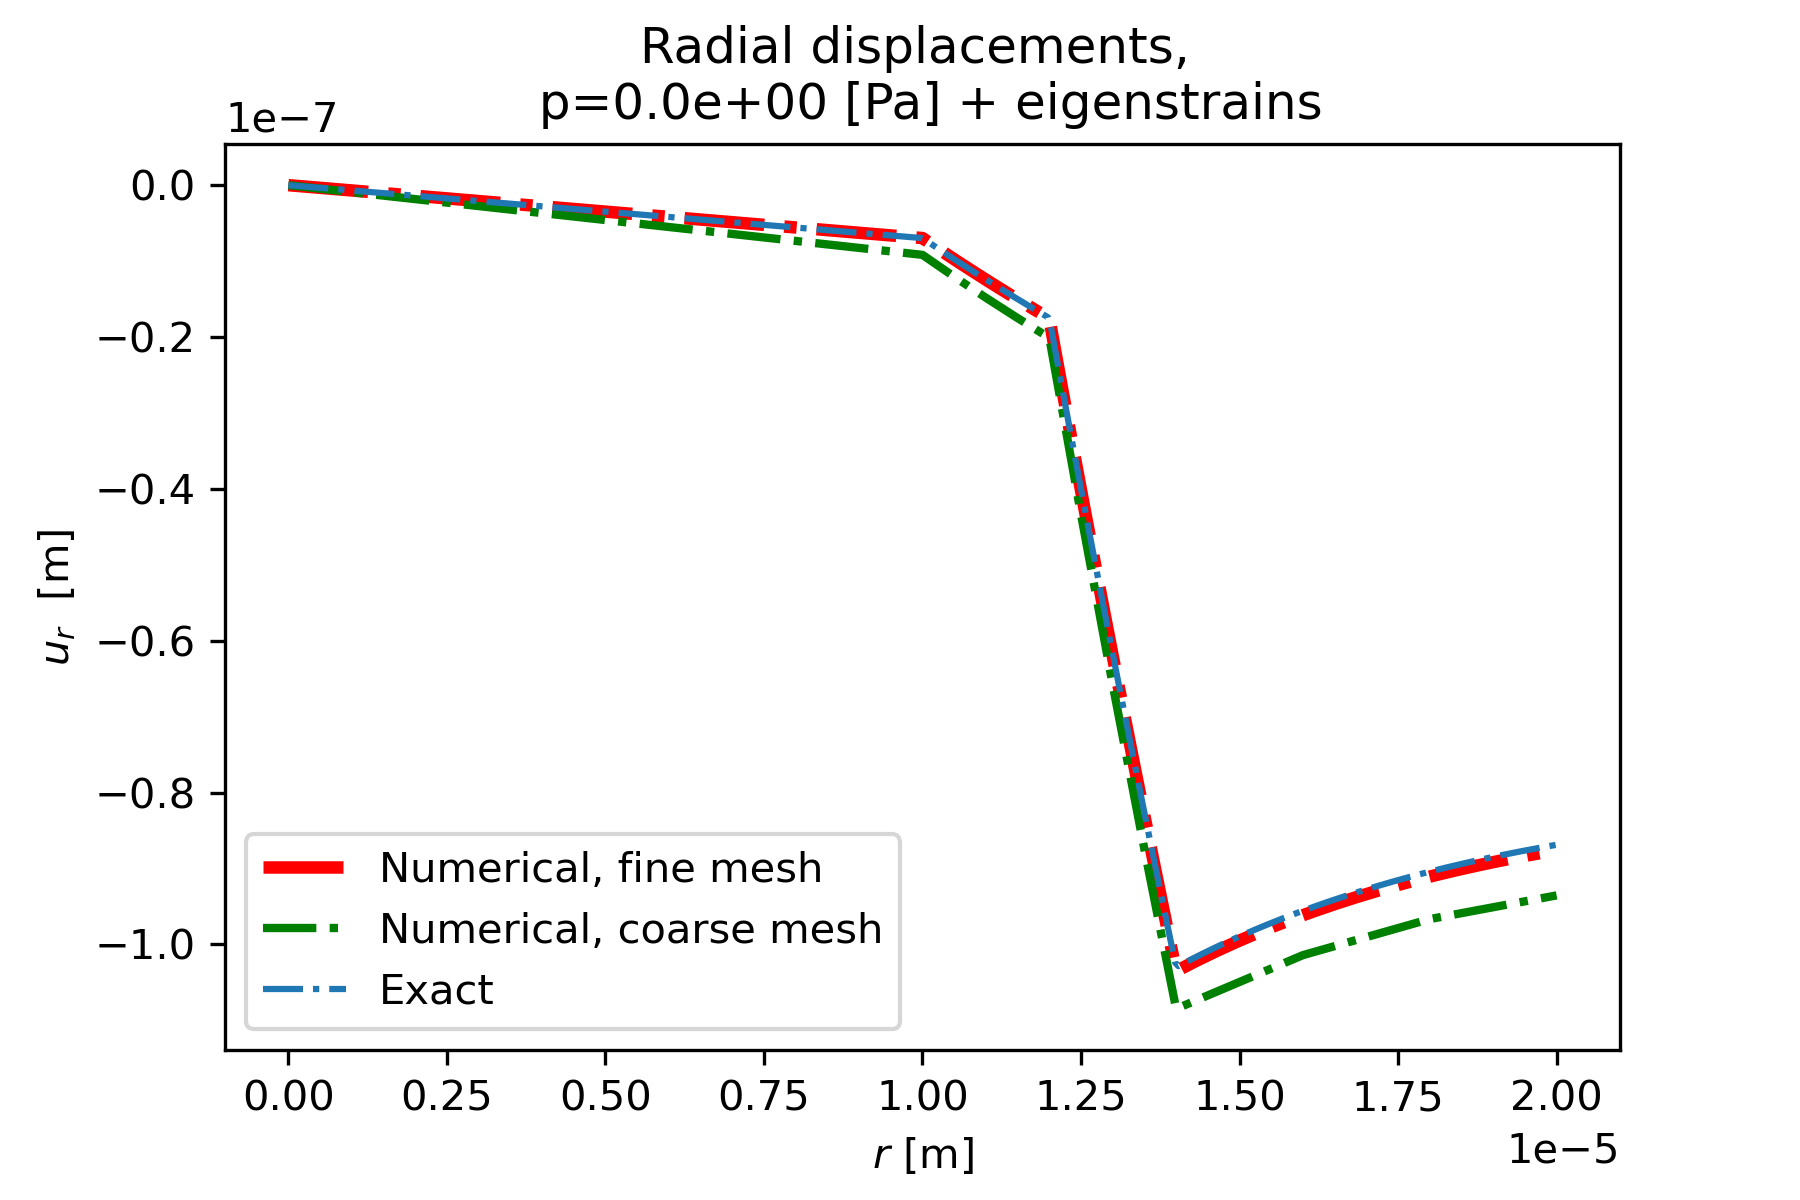
\includegraphics[width=1.\linewidth]{images/Eigenstrains.png}} 
\end{minipage}
\hfill
\begin{minipage}[h]{0.5\linewidth}
\center{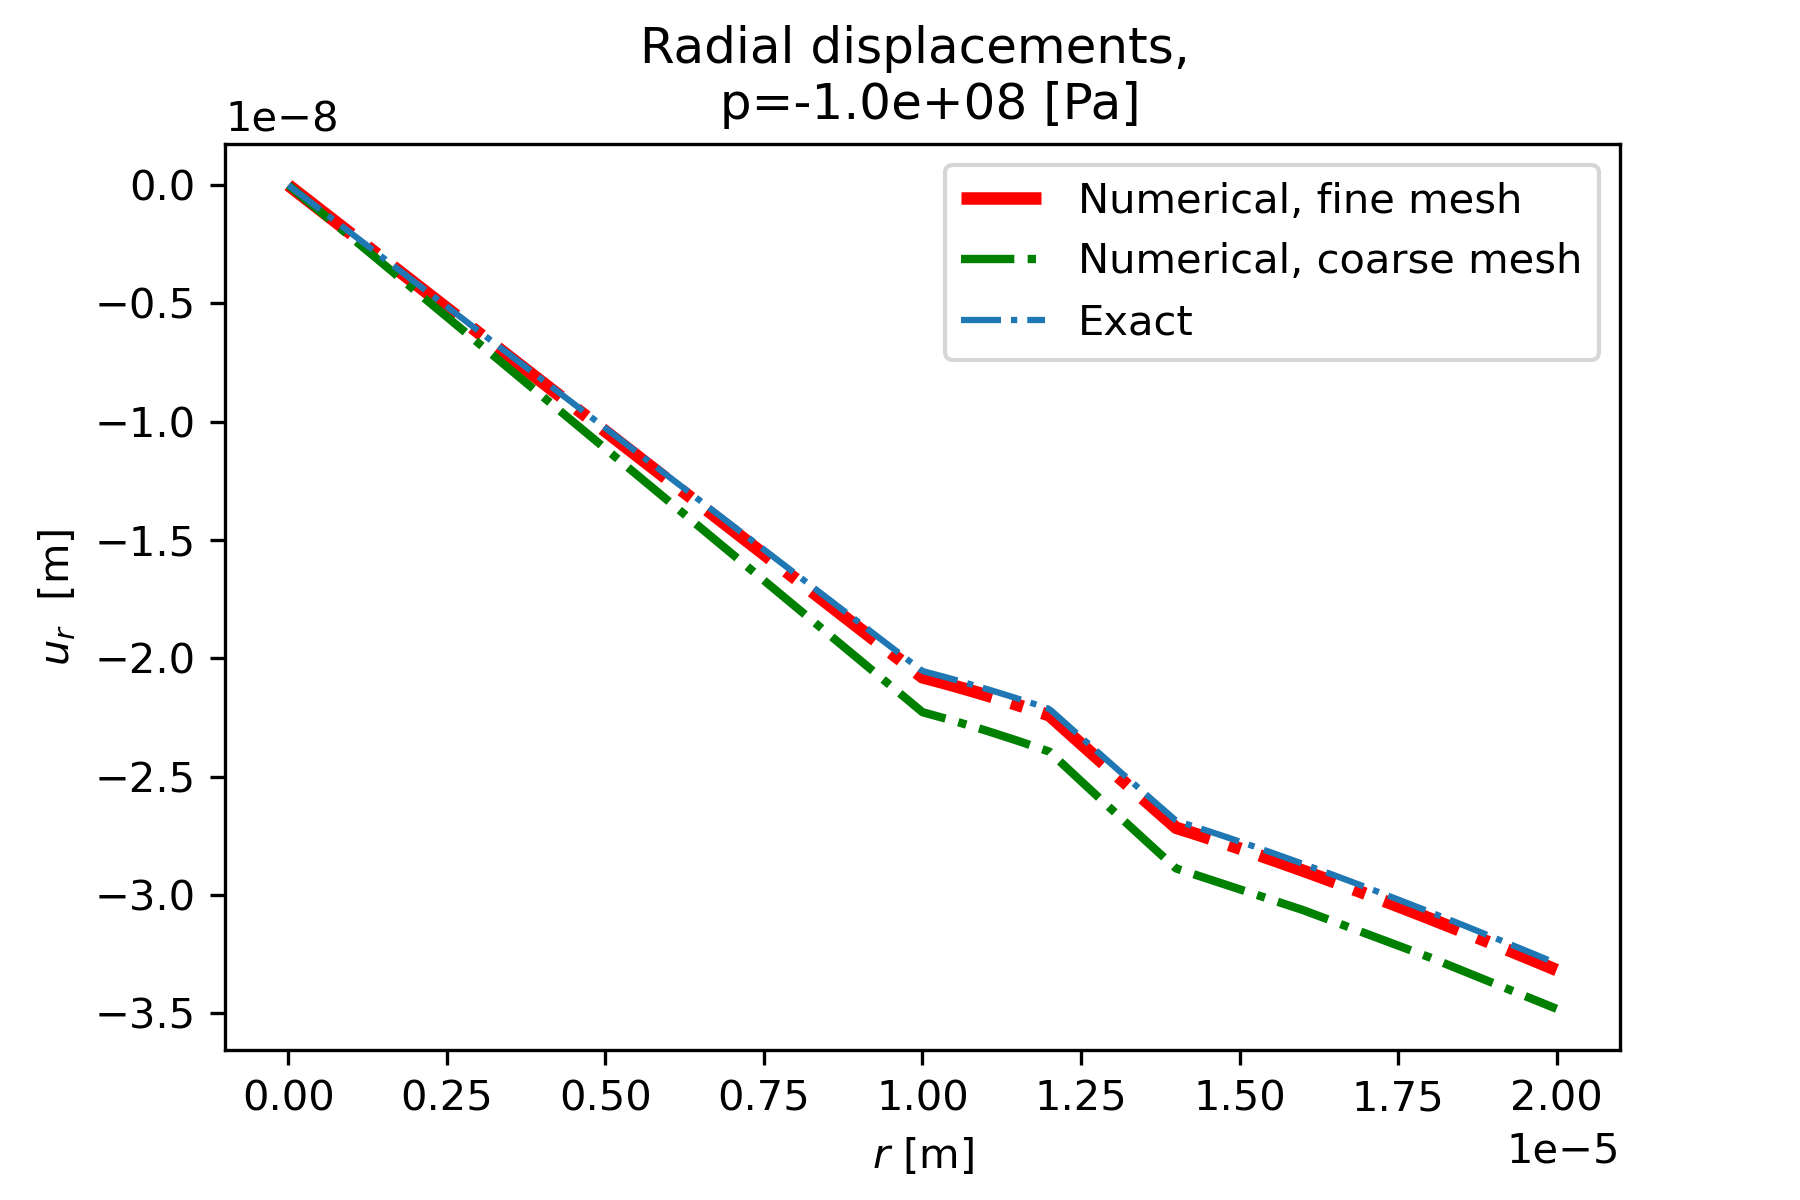
\includegraphics[width=1.\linewidth]{images/PressureDifferent.png} }
\end{minipage}
\caption{Comparison with exact solution. Eigenstrains (left), External pressure (right).}
\end{figure}

\subsubsection{Pressure effect on phase evolution.}

To see the effect of the pressure, hydrostatic pressure to be computed from the mechanical problem. Hydrostatic pressure is close to its average inside each phase. Therefore, diffusion coefficients were updated with averages of hydrostatic pressure, which allows for keeping diffusion coefficients homogeneous inside each phase. 

Three different cases for phase kinetics were considered:  1) Eigenstrains influence only. 2) External pressure. 3) External tension.%1) No pressure effect on phase kinetics. 2) Eigenstrains influence only. 3) External pressure. 4) External tension.

\begin{figure}[h]
\begin{minipage}[h]{0.5\linewidth}
\center{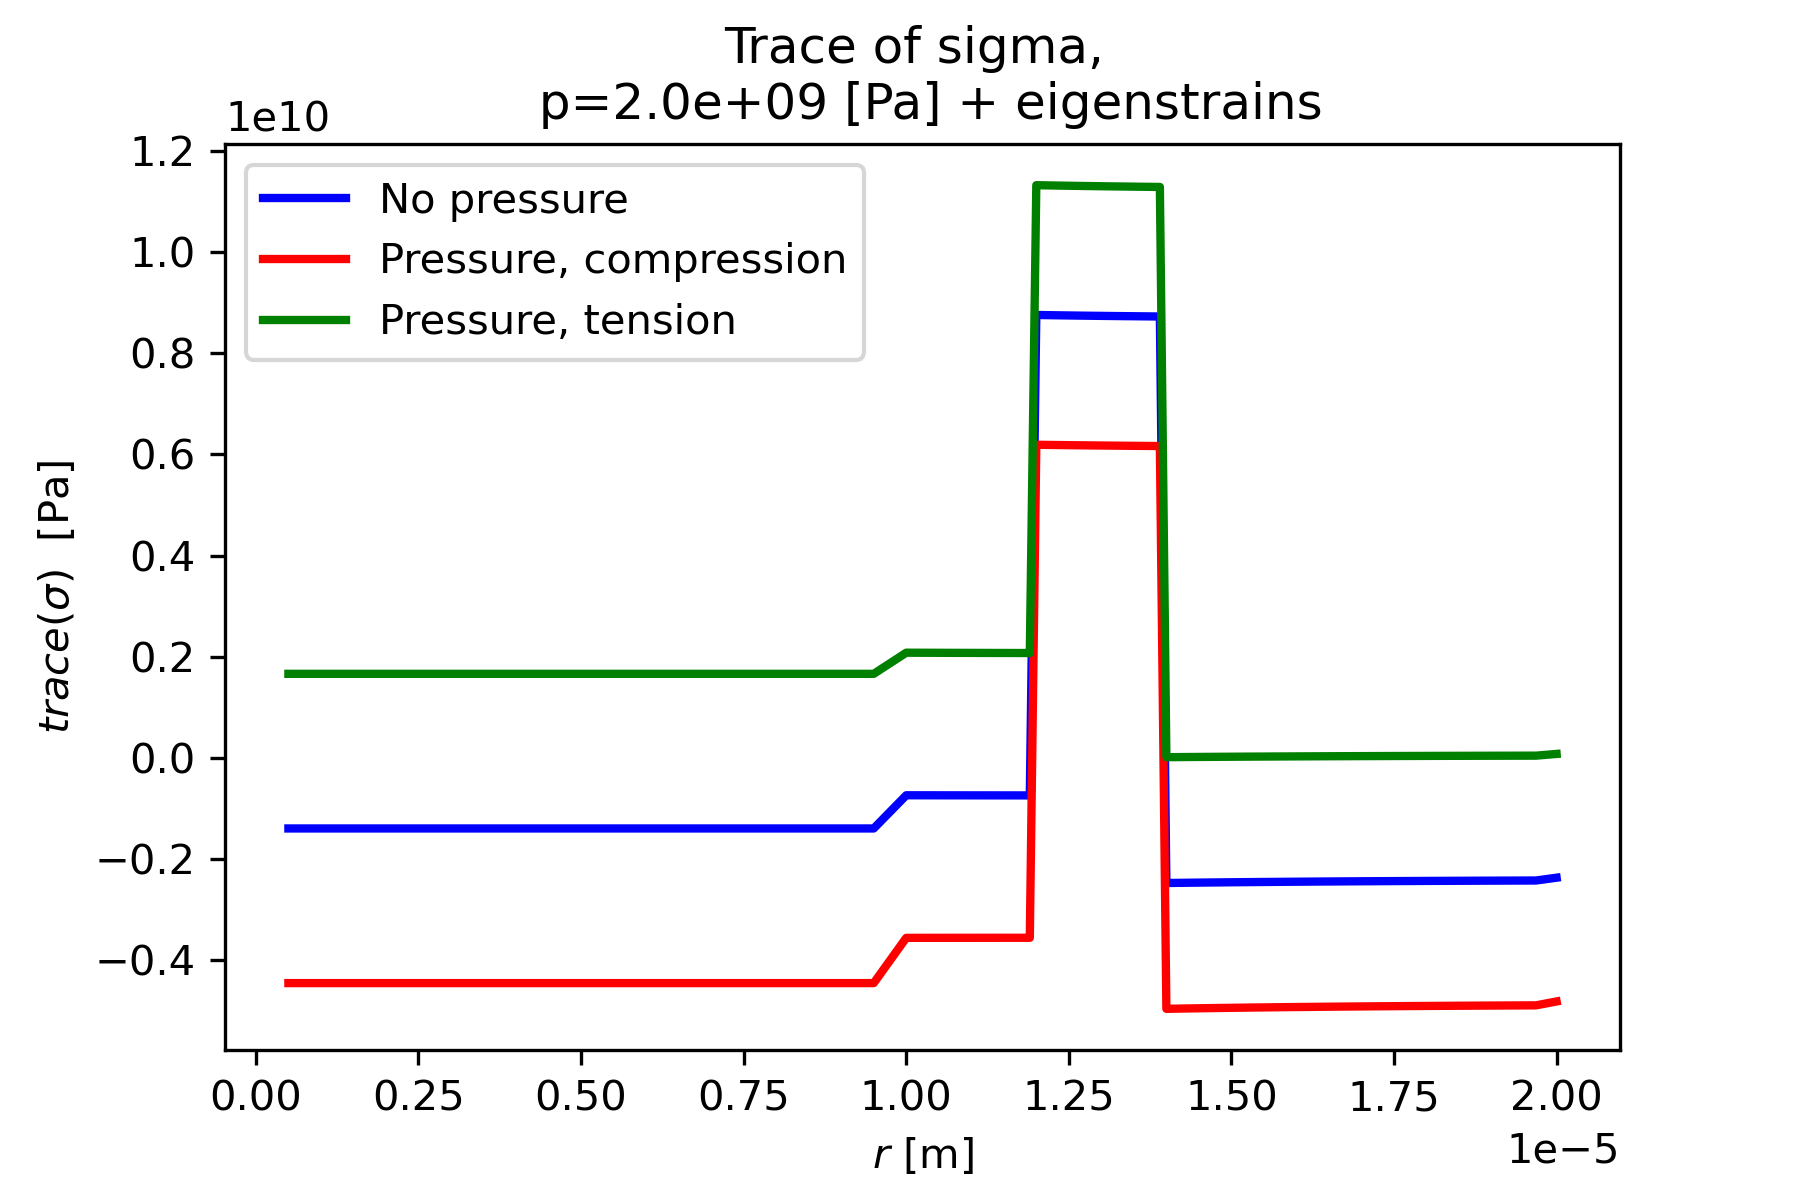
\includegraphics[width=1.\linewidth]{images/Trace.png} }
\end{minipage}
\hfill
\begin{minipage}[h]{0.5\linewidth}
\center{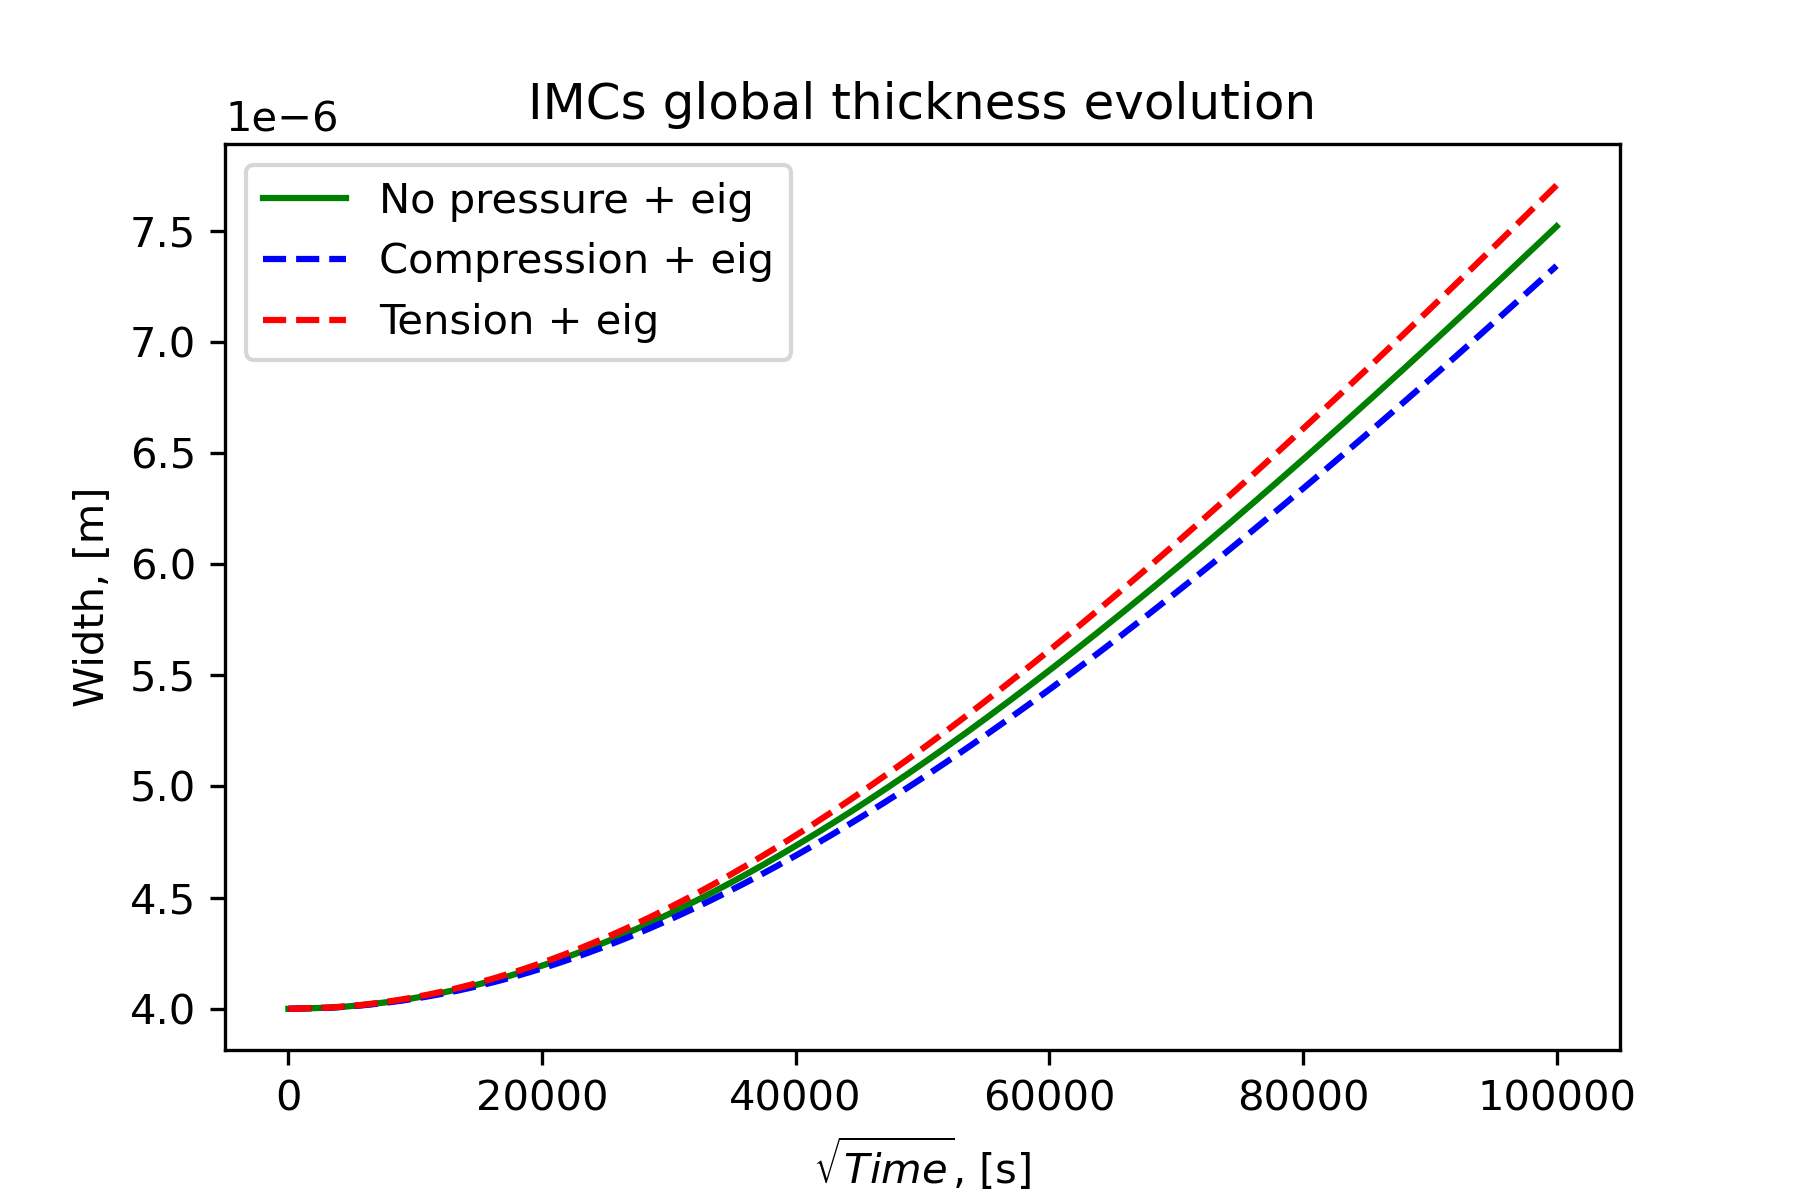
\includegraphics[width=1.\linewidth]{images/StressEffect.png} }
\end{minipage}
\vspace{-2.5em}
\caption{ Stress effect on phase kinetics. $k = 1.0e-7$ }
\end{figure}

As can be seen from the numerical results, external pressure decreases the growth of the intermetallics, while external tension make an opposite effect and increases the growth.

\section{Conclusions}

A 1d multiphase diffusion model was implemented to analyze the growth of intermetallics in Cu-Sn binary system. The model allows to take into account diffusion controlled growth of phases and influence of external pressure on diffusion coefficients. Some serious assumptions were made to simplify calculations. This model can be useful for estimation of phase kinetics inside $Nb_3 Sn$ superconducting wire. 

%The comparison between modelling and experimental observations from the lit

\begin{thebibliography}{}
\bigskip
\bibitem{Erickson1994} Erickson KL, Hopkins PL, Vianco PT (1994) Solid-state intermetallic
compound growth between copper and high-temperature, tinrich solders-Part II--modeling. J Electron Mater 23(8):729-734

\bibitem{Mei1992} Mei Z, Sunwoo AJ, Morris JW (1992) Analysis of low-temperature
intermetallic growth in copper-tin diffusion couples. Metall
Mater Trans A 23(3):857-864

%\bibitem{Cheng2015}  Cheng, Ya-Chi, et al. "Effect of loading stress on the growth of Cu/Sn intermetallic compounds at high temperatures." Journal of Electronic Materials 44.1 (2015): 604-611.

%\bibitem{Huang2009}  Huang, Zhiheng, Paul P. Conway, and Rongshan Qin. "Modeling of interfacial intermetallic compounds in the application of very fine lead-free solder interconnections." Microsystem technologies 15.1 (2009): 101.
\end{thebibliography}


\newpage
\section{Additional notes}

If the initial concentration profile is constant, than there will be no flux, and the interfaces will not move with time. However, in reality the diffusion will occur. In that case, there will be no chemical equilibrium at the interfaces at the beginning of the process. As some of the tin will penetrate through all the IMCs and reach copper, the chemical reaction will occur and after some time (if the rate is much faster then diffusion) the system will reach local chemical equilibrium.
So, summarizing, in case of constant initial profile, boundary conditions for chemical equilibrium should be omitted for initial period of time. 

To compute concetration in each region more precisely, analytical solution for diffusion equation can be used:
$$ c_i = A_i - B_i \; erf(\dfrac{x}{2 \sqrt{D_i t}}),  $$
where $A_i, B_i$ to be computed from boundary conditions at the interfaces. It describes cnahge in concentration with time. It's possible to estimate initial concentration distibution in phases usign that solution with some additional data from experiments.

Here we do no take into account cylindrical geometry. Diffusion eqation is decribed in 1d as for planar interfaces. In cylindrical coordinates, the diffusion equation will slightly change. This geometry issue is to be considered in the future.

Elastic strains and eigenstrains are making an impact on total thickness of the layer. We neglect this effect here.


\section{My notes}

In cylindrical coordinates, diffusion equation for each phase takes form:
$$ \dfrac{\partial c}{\partial t} = \dfrac{1}{r}\dfrac{\partial}{\partial r}(r\dfrac{\partial c}{\partial r}) $$

\noindent If we have a steady state diffusion profile, then the solution is of the form
$$ c = A + B \;ln(r) $$
One have to be careful with boundary conditions, cause when the radius tends to zero, logarithm tends to minus infinity.

It's reasonable, that in our case, we have a zero flux boundary condition at $r=0$. Thus, the concentration profile is constant in Sn phase region. 

However, on the external boundary such type of condition is questionable. There are several possibilities.

There is no saturation on the copper side, because of the big difference in diffusion constants.  For copper flux to make an impact on diffusion, the size of the copper region has to be very low. Estimates has shown that the size of the copper phase is proportional to $e\text{-}15$, to make an comparable impact on fluxes.

To see such an effect, I have to take an extra small time step. Plus, such a small scale is just unphysical.

\end{document}

